\begin{block}{synthesizing pdfs for decision relevance}
    While comparing results across many PDFs is a valuable exploratory exercise (see, \eg, \cref{fig:tradeoffs}), providing end users (\eg, households practicing engineers, and planning departments of local governments) with many PDFs may lead to confusion, inconsistency, and potentially liability (see refs.~\cite{schneider_dangerous:2001,schneider_scenarios:2002}).
    \begin{framed}
        \begin{figure}
            \centering
            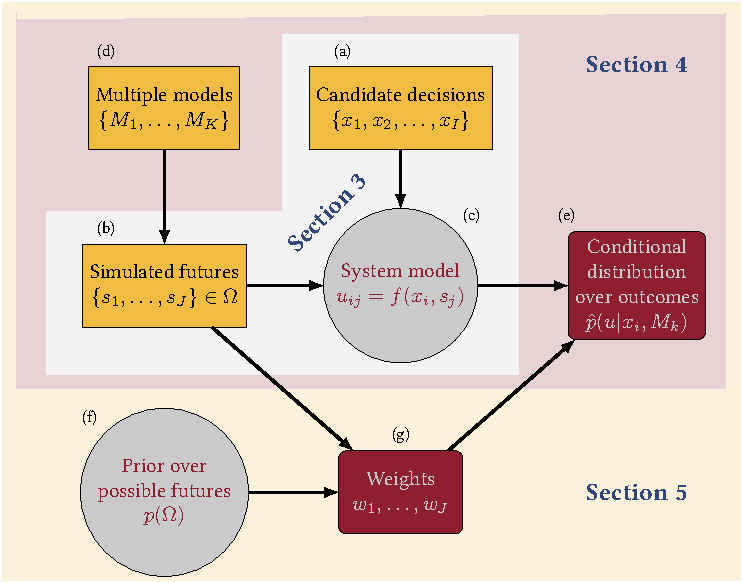
\includegraphics[width=0.8\textwidth]{bayes-rdm.pdf}
            \caption{
                ``Prior Model Averaging'' framework.
            }\label{fig:flowchart}
        \end{figure}
    \end{framed}
    Our approach to synthesizing PDFs is designed for the common case of assessing decisions using simulations (SOWs) from each of $K$ PDFs.
    A system model $(f)$ quantifies the performance $(u)$ of a decision ($x$) under a single SOW ($s$).
    To synthesize, we weight PDFs using an approach based on Bayesian Model Averaging \cite{wong_surge:2018,Yao:2018bu}.
\end{block}